 % File folder with archived pages
% Author:	Leo Arnold
% Contact:	tex@arney.de
% License:	CC BY-SA 3.0
%\documentclass{article}
%\usepackage{tikz}
%\begin{document}

% Scale to your needs
\scalebox{0.1}{
  % All measures in centimeters
  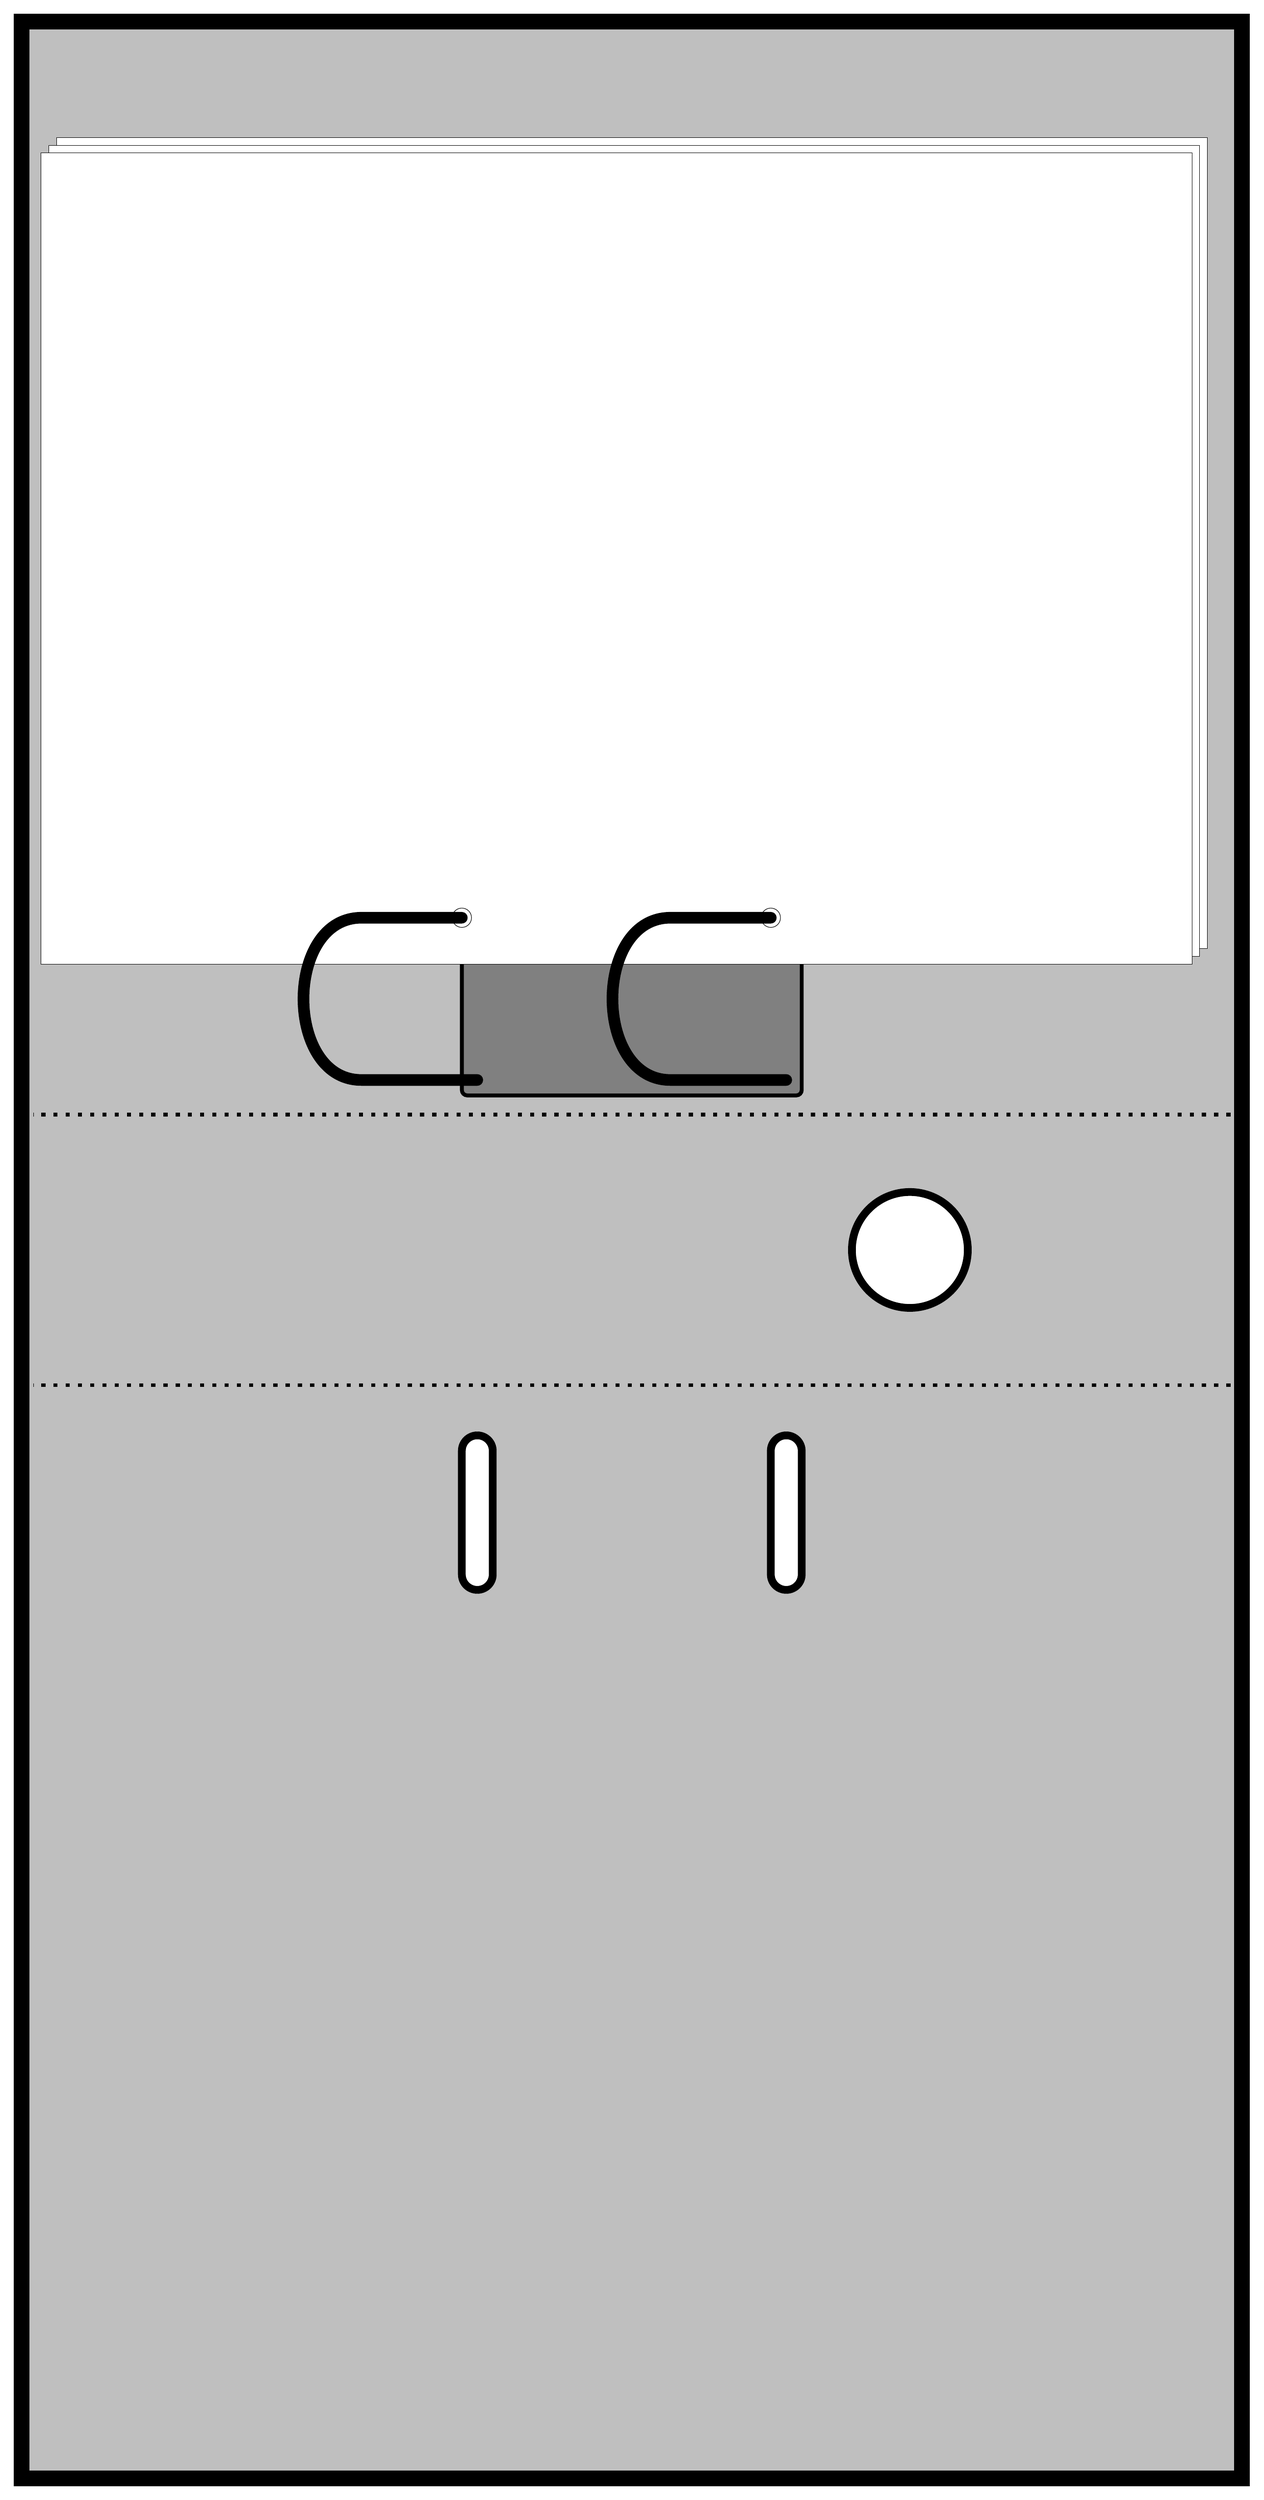
\begin{tikzpicture}[rotate=90]
    % Basic cardboard
    \draw[fill=black]
      (-32,0) rectangle (32,32);
    \draw[fill=gray!50]
      (-31.6,0.4) rectangle (31.6,31.6);

    % Fold lines
    \foreach \i in {-1, 1} {
      \draw[loosely dashed, line width=1mm]
        (\i*3.5,0.5) -- (\i*3.5,31.5);
    }

    % Finger hole
    \draw[fill=white, line width=2mm]
      (0,8.8) circle (1.5);

    % Metal plate
    \draw[fill=gray, line width=1mm, rounded corners]
      (4,11.6) rectangle (9,20.4);

    \foreach \i in {0, 1, 2} {
      % Filed pages
      \draw[fill=white, very thin, shift={(-\i*0.2,\i*0.2)}]
        (7.8,1.1) rectangle (28.8,30.9);
      % Punched holes
      \draw[fill=white, shift={(-\i*0.2,\i*0.2)}]
        (9,12) circle (0.25);
      \draw[fill=white, shift={(-\i*0.2,\i*0.2)}]
        (9,20) circle (0.25);
    }

    \foreach \i in {0, 1} {
      % Metal skewers
      \draw[line cap=round, line width=3mm, shift={(0,\i*8)}]
        (4.4,12) --
        (4.4,15) to [controls=+(90:2) and +(90:2)] (8.6,15)
         -- (8.6,12.4);
      % Holes opposite to skewers
      \draw[fill=white, line width=2mm, rounded corners=4mm, shift={(0,\i*8)}]
        (-8.8,11.6) rectangle (-4.8,12.4);
    }
  \end{tikzpicture}
}

%\end{document}
